\documentclass[a4paper]{report}
\usepackage{tikz}
\usepackage[utf8]{inputenc}
\usepackage{amssymb}
\usepackage{amsmath}

\usetikzlibrary{arrows}

\title{Architecture\\GRT}

\begin{document}
\chapter{DPO graph rewriting approach}
Given a rule $L \overset{l}{\leftarrowtail} K \overset{r}{\rightarrowtail} R$ and a graph $G$, the DPO approach to graph rewriting is to commute the following diagram

\begin{center}
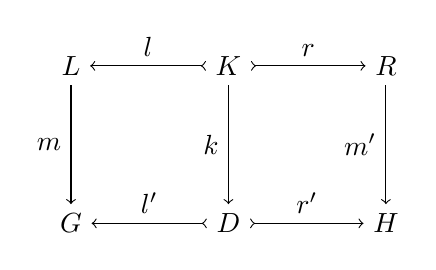
\begin{tikzpicture}
	\node (L) at (0,2) {$L$};
	\node (K) at (2,2) {$K$};
	\node (R) at (4,2) {$R$};
	\node (G) at (0,0) {$G$};
	\node (D) at (2,0) {$D$};
	\node (H) at (4,0) {$H$};

	\path[>->] (K) edge node [above] {$l$} (L);
	\path[>->] (K) edge node [above] {$r$} (R);
	\path[>->] (D) edge node [above] {$l'$} (G);
	\path[>->] (D) edge node [above] {$r'$} (H);
	\path[->] (R) edge node [left] {$m'$} (H);
	\path[->] (L) edge node [left] {$m$} (G);
	\path[->] (K) edge node [left] {$k$} (D);
\end{tikzpicture}
\end{center}
in which both squares are pushouts.

The morphisms in this diagram are:
\begin{itemize}
	\item $m$: is a homomorphism detection algorithm. In the diagram, $m$ is a single homomorphism, non-deterministically detected, but ideally, the algorithm should return all possible homomorphisms from $L$ to $G$. It is calculated.

	A second view of such morphism is that it is the set of arrows that maps $a \mapsto b, a \in L, b \in G$.

	\item $l, l', r, r'$ are all inclusions (supose that each one of them can be generically identified by $\phi : S \to T$). $\phi$ can be defined as the identities of the elements of the graph $T \backslash S$, and the inverse morphism $\phi^{-1}: T \nrightarrow S$ is a partial morphism that excludes nodes and edges in $T \backslash S$.

	\item $k, m'$: are morphisms derived from $m$. $k$ has the arrows of $m$ which the source is removed by $l^{-1}$ removed, along with the target of such arrows. $m'$ adds arrows to $k$, with source in the elements of $R \backslash K$ and target in the elements of $H \backslash D$.
\end{itemize}

These are all structure preserving. Two conditions impede the transformation to be applied:
\begin{itemize}
	\item \textit{dangling condition}: If after the deletion of a node, an edge is left ``dangling'', i.e. the node deleted was the source or target of an edge that was not removed.
	\item \textit{identification condition}: if an element is both deleted and maintained.
\end{itemize}

\chapter{Representation and algorithms}
\section{Graph}
A graph is represented by two sets $V$ of vertices and $E$ of edges. Each element must have an numerical identity. Edges must contain also a pair of node identites that are the source and target of an edge.

A morphism between graphs is represented by two lists of pairs: node and edge identities. The first element is the source of the morphism and the second element is the target of the morphism. one of them can be $\bot$ (\texttt{Nothing}), meaning that the element is created (when in the source) or deleted (when in the target). For the DPO approach, the source of each pair must be unique, except for $\bot$. This morphism allows to describe a span $L \overset{l}{\leftarrowtail} K \overset{r}{\rightarrowtail} R$ as follows.
\begin{itemize}
	\item $L$ are all sources $s$ that are mapped to $\bot$ ($s \mid s \mapsto \bot$), plus all that are maintained ($s \mid s \mapsto s$).
	\item $R$ are all targets $t$ that are mapped from $\bot$ ($t \mid \bot \mapsto t$), plus all that are maintained ($t \mid t \mapsto t$).
	\item $K$ are all item that are maintained ($k \mid k \mapsto k$).
	\item $l$ are all pairs that the target is $\bot$ ($(s, \bot) \mid s \mapsto \bot$).
	\item $r$ are all pairs which the source if $\bot$ ($(\bot, t) \mid \bot \mapsto t$).
\end{itemize}
\end{document}